查看本节演示代码：\democode{05}{5.8_Reinforcement_Learning} \ \democodegithub{05}{5.8_Reinforcement_Learning}

\subsubsection{背景}

一个完整的强化学习算法（Reinforcement Learning, RL）由智能体（Agent）、环境（Environment）、状态（State）、动作（Action）和奖励（Reward）组成。智能体执行一个动作后，环境会根据该动作转移到新的状态，并依据一定规则给出奖励。随后，智能体根据获得的新状态和奖励更新其决策过程并给出新的动作，如此循环，直到整个控制过程完成 \cite{kaelbling1996reinforcement}。我们用 $\pi_{\theta}$ 表示策略函数，$s$ 表示环境的每个状态，$r$ 表示每个状态中的奖励，$a$ 表示智能体的动作。RL 的架构如图 \ref{RL_frame} 所示。
\begin{figure}[ht]
  \centering
  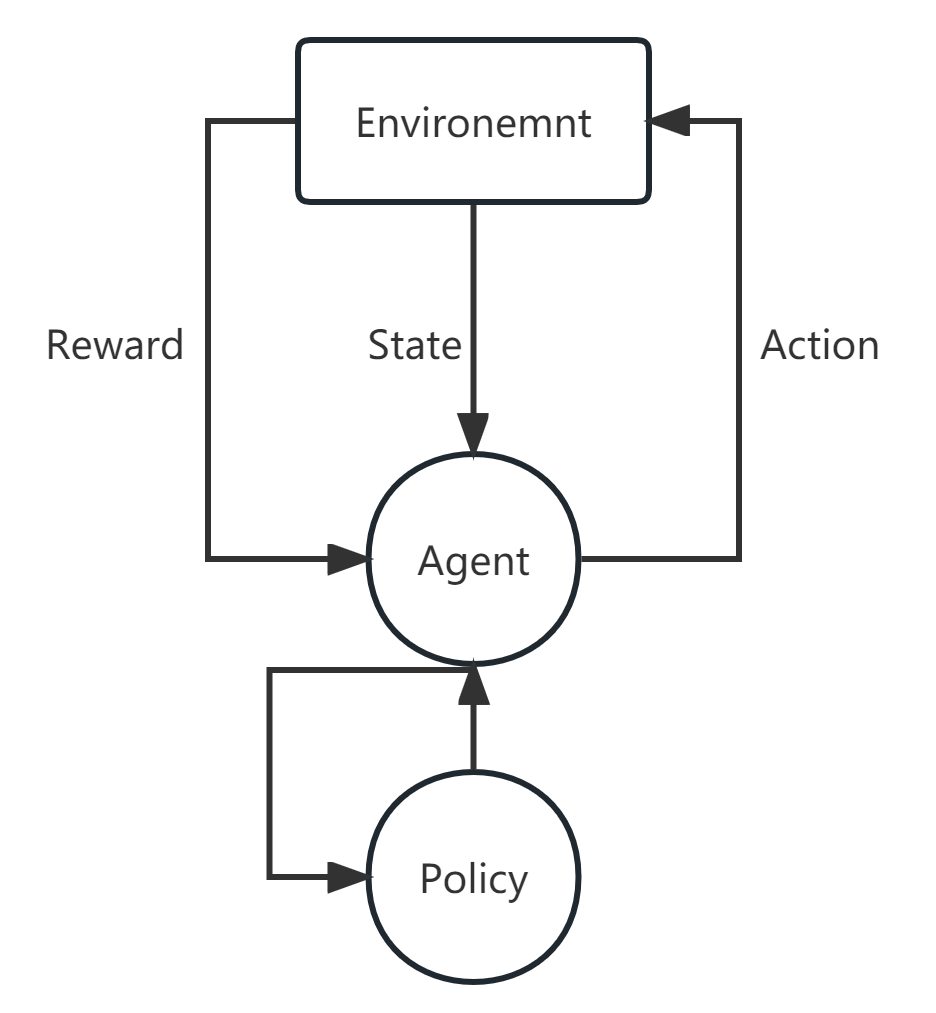
\includegraphics[scale=0.4]{5.4.5_RL/RL.png}
  \caption{\label{RL_frame} RL 工作流程示意图。}
\end{figure}

假设一个环境包含 $N$ 个不同状态。我们在状态 $s_{i-1}$ 上执行动作 $a_{i-1}$，并得到结果状态 $s_i$。从状态 $s_i$ 在动作 $a_i$ 下转移到状态 $s_{i+1}$ 的转移概率函数可以写为 $P(s_{i+1}|s_i,a_i)$。同时，每个状态中都有一个由奖励函数 $R_i=R(a_i,s_i,s_{i-1})$ 计算得到的奖励 $r_i$。在环境变化过程中，如果奖励期望只由最新的 $state$ 决定，则称其为马尔可夫决策过程。因此，智能体选择每条 $T$ 步轨迹的概率为：

\begin{equation}
    \begin{split}
        &P(\tau|\pi_{\theta})=\\
        &\rho(s_0)\prod_{k=0}^{k=T-1}P(s_{k+1}|s_{k},a_{k})\pi_{\theta}(a_{k}|s_{k}),
    \end{split}
\end{equation}
其中 $\rho$ 是初始状态分布。于是，$T$ 步轨迹奖励的期望为：
\begin{equation}
    \eta(\pi_{\theta})=\int_{\tau}P(\tau|\pi_{\theta})R(\tau)d\tau.
\end{equation}
为了得到最优策略函数 $\pi_{\theta}$，需要训练智能体来最大化期望 $\eta$，即：
\begin{equation}
    \pi_{\theta}^{opt}=\mathrm{argmax}_{\theta}\eta(\pi_{\theta}).
\end{equation}
在后续部分中，我们将展示如何在量子设备上训练智能体。

\subsubsection{混合深度 Q 网络}

用量子变分线路替换经典深度 Q 网络智能体中的神经网络，即可得到混合深度 Q 网络（Hybrid Deep Q-Network, HDQN）\cite{Q_rl}。HDQN 的架构如图 \ref{HDQN} 所示。

\begin{figure*}[ht]
    \centering
    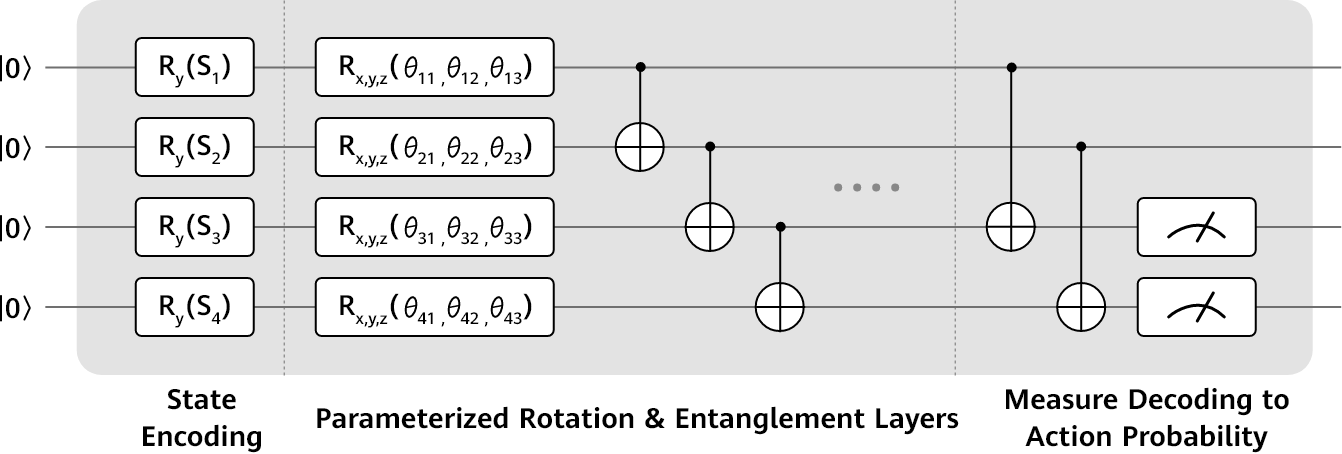
\includegraphics[width=0.9\linewidth]{5.4.5_RL/HDQN.png}
    \caption{\label{HDQN} HDQN 架构。}
  \end{figure*}

我们通过经典神经网络计算参数 $\theta$，并用这些参数构造量子变分线路。最终，量子部分会向环境施加动作，同时环境返回奖励 $r_i$。记 $e_i=(s_i,a_i,r_{i+1},s_{i+1})$ 为一条经验。在训练阶段，我们会把这些经验作为训练样本，并依据损失函数 $L(\theta)$ 调整经典部分和量子部分中的参数：
\begin{equation}
\begin{split}
    L(\theta_{j})=&E[R_{i+1}+\\
    &\gamma \max_{\alpha^{'}}Q(s_{i+1},a^{'},\theta_{j}^{-})-Q(s_{i},a_{i},\theta_{i})^2].
\end{split}
\label{loss func}
\end{equation}

\textit{变分量子线路} -- 变分量子线路是一类使用可调参数的量子线路，这些参数可以随外部环境改变。在这里，我们根据文献 \cite{Q_rl} 中的架构，采用 encoder 与 ansatz 组合的方式构造量子线路。其中，ansatz 采用 Hardware Efficient 线路。整体量子线路如图 \ref{Agent_qc} 所示。

\begin{figure*}[ht]
  \centering
  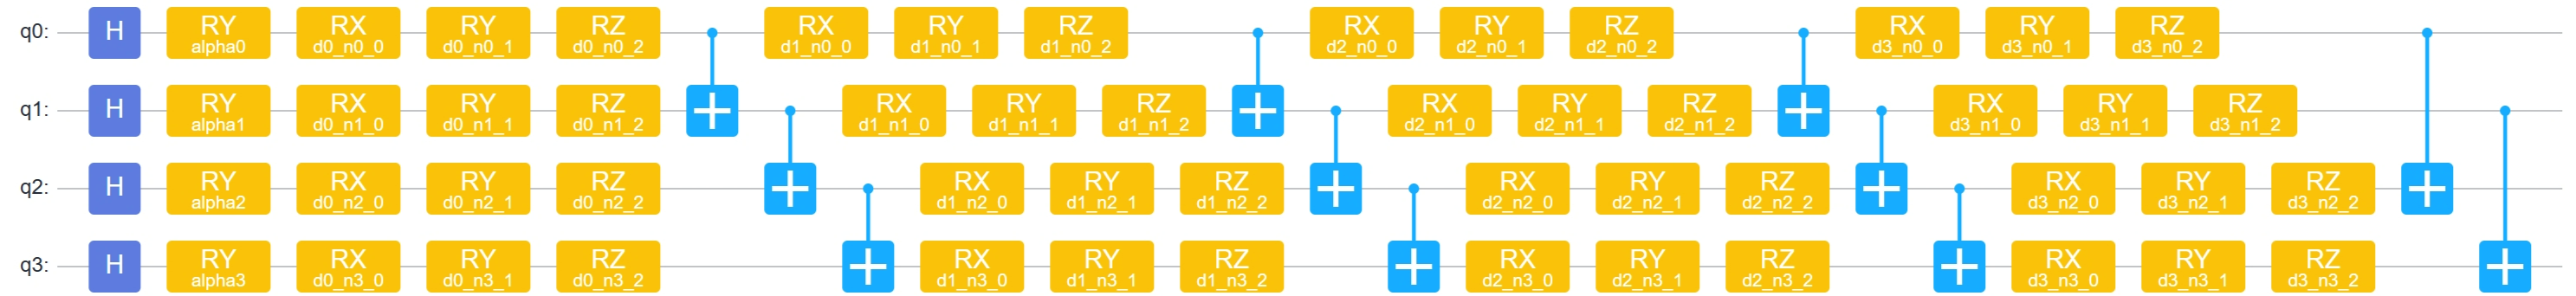
\includegraphics[scale=0.5]{5.4.5_RL/Circuit.png}
  \caption{\label{Agent_qc} RL 智能体的整体量子线路。}
\end{figure*}

\textit{MindQuantum 中的实现} -- 这里给出使用 \MindQuantum\ 实现 HDQN 的示例。第一步是构造包含 encoder 和 ansatz 的量子变分线路。
\begin{lstlisting}
def __get_encoder(self):
    encoder = Circuit()
    encoder += UN(H, 4)
    for i in range(4):
        encoder += RY(f'alpha{i}').on(i)
    encoder = encoder.no_grad()
    # 无梯度量子线路: no_grad()
    encoder.summary()
    return encoder
def __get_ansatz(self):
    ansatz = HardwareEfficientAnsatz\\
        (4, single_rot_gate_seq=[RX,RY,RZ],\\
        entangle_gate=X, depth=3).circuit
    ansatz += X.on(2,0)
    ansatz += X.on(3,1)
    ansatz.summary()
    return ansatz
self.circuit = self.encoder + self.ansatz
\end{lstlisting}

经过量子线路处理后，我们需要构造一个可观测量哈密顿量作为测量基。这里仅在 $\sigma_y$ 基上测量第二个和第三个量子比特。哈密顿量如下：
\begin{equation}
    H=I\otimes I\otimes\sigma_y\otimes\sigma_y.
\end{equation}
我们可以用 \MindQuantum\ 按如下方式构造该哈密顿量：
\begin{lstlisting}
def __get_observable(self):
    hams=[Hamiltonian(QubitOperator(f'Y{i}'))\\
        for i in [2, 3]]
    return hams
\end{lstlisting}
此外，通过 \getexpectationwithgrad 函数可以方便地获得期望值并计算期望值梯度，该梯度可用于优化参数。

接下来，需要实现经典部分，即一个带激活函数的三层全连接神经网络。
\begin{lstlisting}
class Critic(nn.Cell):
    def __init__(self):
        super(Critic, self).__init__()
        self.relu = nn.ReLU()
        self.fc1 = nn.Dense(4, 64)
        self.fc2 = nn.Dense(64, 256)
        self.fc3 = nn.Dense(256, 1)

    def construct(self, x):
        x = self.relu(self.fc1(x))
        x = self.relu(self.fc2(x))
        x = self.fc3(x)
        return x
\end{lstlisting}

\textit{环境} -- 这里关注 gym 游戏 \code{"CartPole-v0"}。该游戏中有一辆在轨道上运动、上方竖立着摆杆的小车。游戏有两个输入 $0$ 和 $1$，分别对应向左和向右两个方向。用户需要控制小车沿这两个方向移动，并尽可能长时间地保持摆杆平衡。

第一步是通过 gym 创建环境。
\begin{lstlisting}
import gym
env = gym.make('CartPole-v0')
\end{lstlisting}
\textit{记忆缓冲区} -- 在训练过程中，训练样本会从之前的经验 $e_i$ 中随机选取。因此，需要构造一个缓冲区来存储并采样经验 $e_i$。
\begin{lstlisting}
class Memory(object):
    ......
\end{lstlisting}

完整实现可见于本节开头给出的示例代码。

\subsubsection{训练}
最后一步是模型训练。首先，用随机参数初始化 HDQN，并让 actor 与环境交互。然后，将交互结果存入记忆缓冲区，作为训练样本。最后，从记忆缓冲区采样，并利用损失函数（\ref{loss func}）同时调整经典部分和量子部分的参数。受篇幅限制，这里不再给出详细代码。

\textit{数值模拟结果} -- 为了评估 HDQN 的效果，我们进行了若干实验。图 \ref{stochastic} 展示了多次实验的平均结果与随机策略实验之间的比较。结果表明，以量子线路作为智能体的强化学习模型确实学习到了策略。
\begin{figure}[ht]
  \centering
  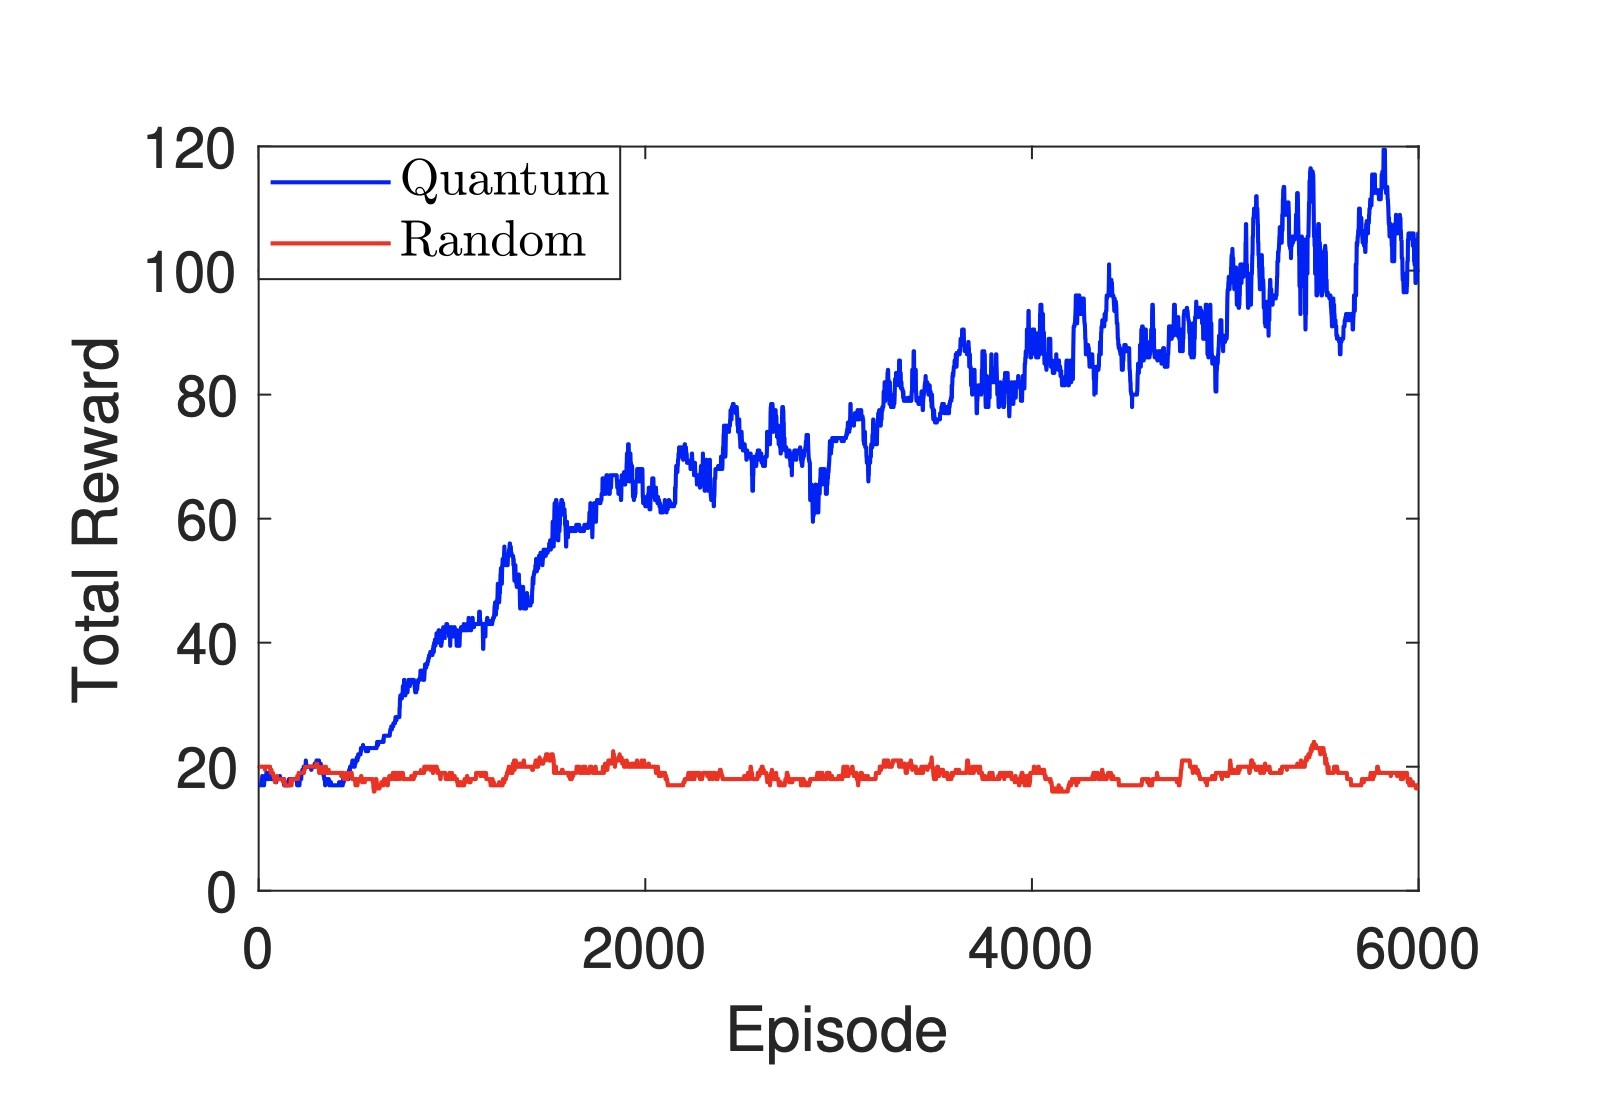
\includegraphics[scale=0.3]{5.4.5_RL/result_paper.jpg}
  \caption{\label{stochastic} RL 与随机策略的比较。}
\end{figure}
